\pdfoutput=1
\RequirePackage{amsmath}
\documentclass{emulateapj}
\usepackage[varg]{newtxmath}
\usepackage{newtxtext}
\usepackage[utf8]{inputenc}
\usepackage{natbib}
\usepackage{microtype}
\usepackage{hyperref}
\graphicspath{ {figs/}, {../}, {../luis-programas}}

\begin{document}

\title{
  Stagnation Pressures of Stationary Bowshocks in the Orion Nebula:\\
  Diagnostics of Inner and Outer Flows  
}
\author{
  William J. Henney, 
  Luis A. Gutiérrez-Soto,
  Jorge A. Tarango-Yong 
}
\affil{Centro de Radioastronomía y Astrofísica,
  Universidad Nacional Autónoma de México, Apartado Postal 3-72,
  58090 Morelia, Michaoacán, Mexico; w.henney@crya.unam.mx, l.gutierrez@crya.unam.mx, j.tarango@crya.unam.mx}

\begin{abstract}
We present a complete catalog of all the stationary emission line arcs (LL objects and proplyd bowshocks) found in archival HST imaging of the Orion Nebula.   The total number of objects detected is 73, of which 20 have not previously been reported in the literature.  We classify the shapes of emission line arcs by fitting conic sections to the inner and outer shell boundaries and calculate the background corrected H alpha surface brightness of each object.   We find significant differences in the shell shapes between the objects closest to the ionizing stars and those farther away.  The closer group, which all represent proplyd interactions with the hypersonic stellar wind, have relatively closed shapes, while the farther group, which are due to interactions with the transonic ionized champagne flow in the nebula, are more open and hyperbolic.  Although some of the latter group are also known proplyds, many are not, and the largest and brightest arcs tend to be associated with particularly luminous young stars, suggesting that the intrinsic T Tauri disk wind may play a role.  The orientations of the arcs, together with the stagnation pressures estimated from the surface brightness, allow the internal velocity field of the H II region to be probed.  We find that approximately radial flows from the core of the nebula dominate over disordered, turbulent flows.
\end{abstract}


\section{Introduction}
\label{sec:intro}

\begin{figure*}
  \centering
  \includegraphics[width=\linewidth]{LL-outer-inner-extend}
  \caption{Inner and outer flows}
  \label{fig:innerouter}
\end{figure*}


\begin{figure}
  \centering
  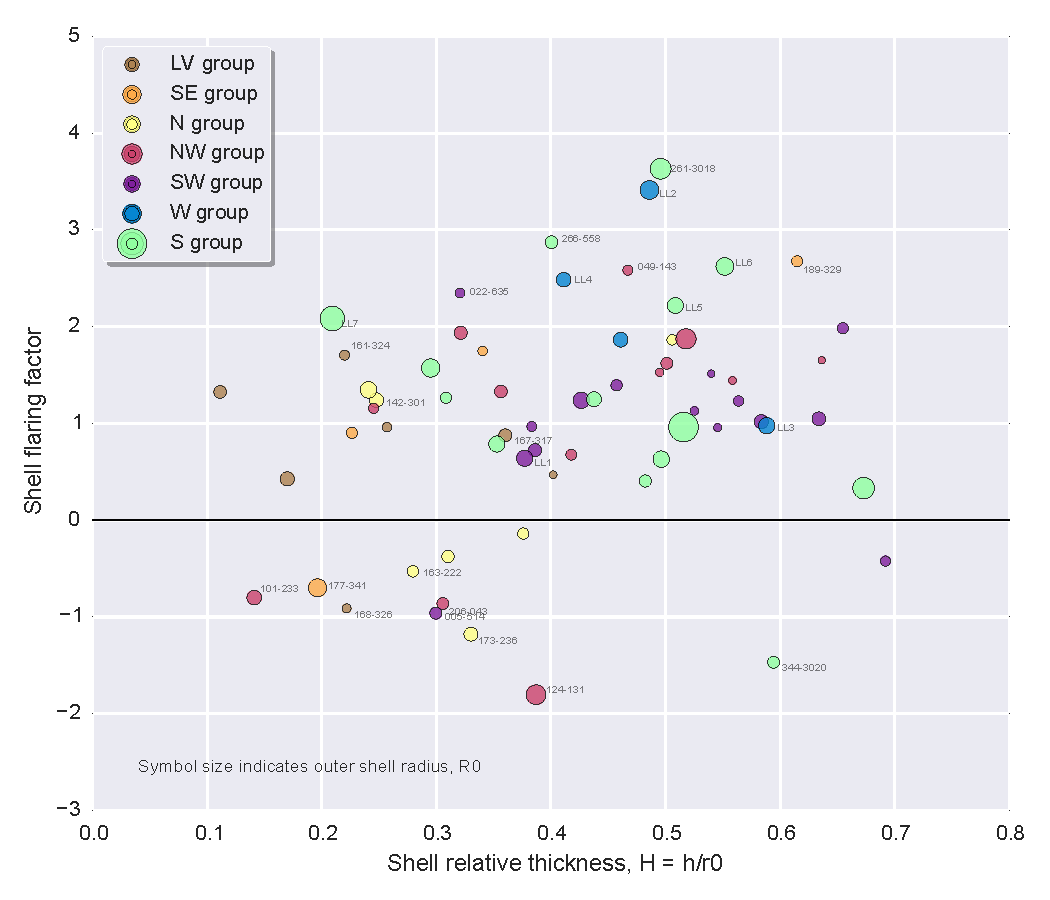
\includegraphics[width=\linewidth]{will-Flare-vs-H-class}
  \caption{The degree of ``flaring'' of the shells (see text) as a
    function of the shell relative thickness.}
  \label{fig:flaring}
\end{figure}


\begin{figure}
  \centering
  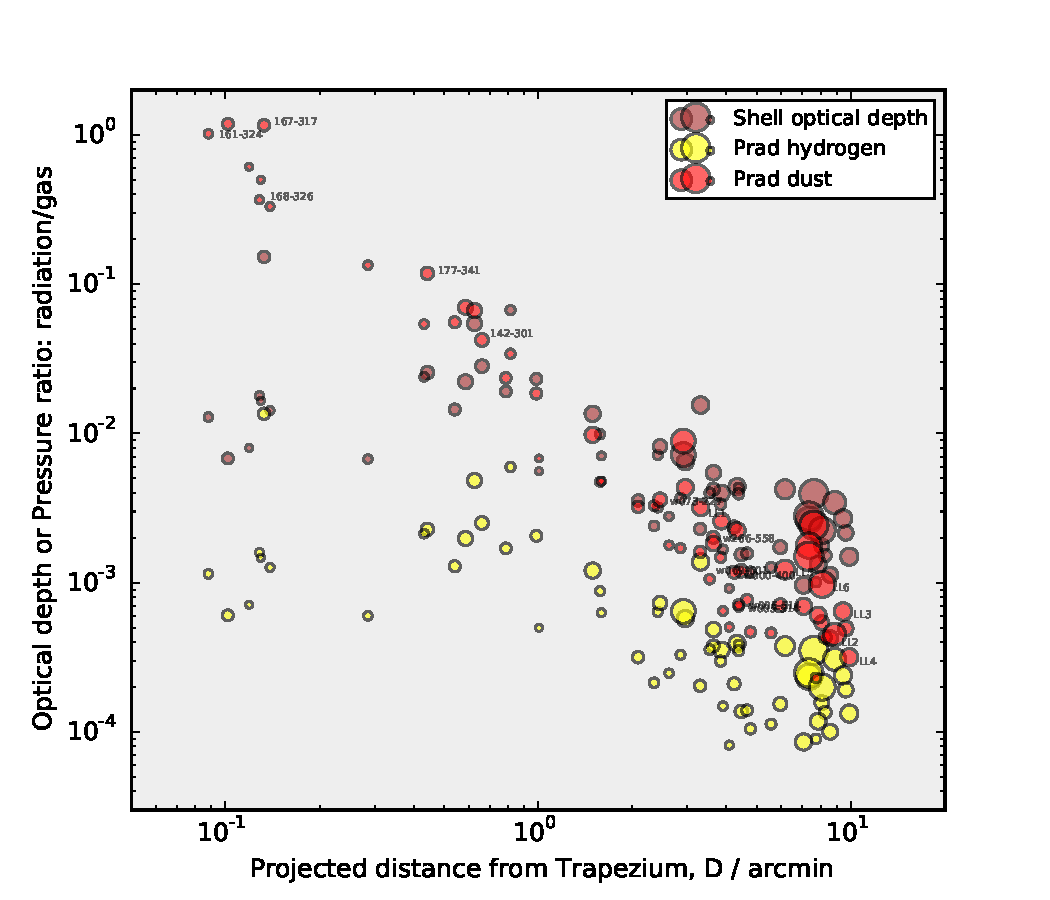
\includegraphics[width=\linewidth]{will-Prad-frac-vs-D}
  \caption{Relative importance of radiation pressure.}
  \label{fig:flaring}
\end{figure}

\begin{figure}
  \centering
  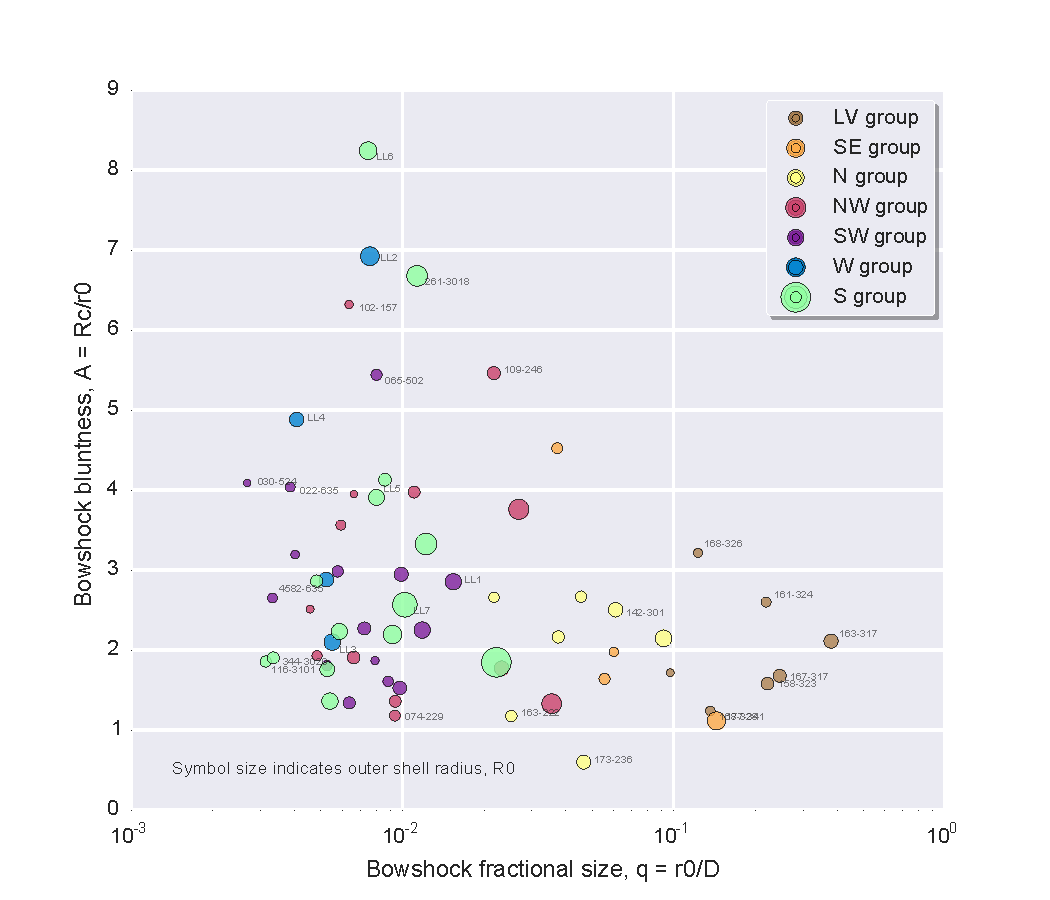
\includegraphics[width=\linewidth]{will-A-vs-q-class}
  \caption{Relative curvature versus relative size.}
  \label{fig:flaring}
\end{figure}

\end{document}
